\documentclass[a4paper,twoside]{report}

\usepackage{listings}
\usepackage{color}
\usepackage{graphicx}
\usepackage{makeidx}

% Use the head environment around method heads
\lstnewenvironment{head}[1]%
{\lstset{frame=topline,emph={#1},emphstyle=\color{blue}\textbf}}%
{}

% Use the parameters environment after heads
\newenvironment{parameters}%
{\begin{tabular}{@{\hspace{2em}}lp{0.6\textwidth}}}%
{\end{tabular}\par\vspace{1mm}\par\hrule\par\vspace{5mm}}

% Use the code environment around method code examples
\lstnewenvironment{code}[1]%
{\lstset{frame=single,caption={#1}}}%
{}

\renewcommand{\lstlistingname}{Example}

%\lstset{language=python,basicstyle=\ttfamily\small}
\lstset{language=python,identifierstyle=\ttfamily}

\newcommand{\cls}[1]{\lstinline|#1|}
\newcommand{\fa}[1]{\lstinline|#1|}
\newcommand{\expr}[1]{\lstinline|#1|}
\newcommand{\ret}{\emph{return value}}
\newcommand{\self}{\emph{self}}

\title{Python-csa tutorial v0.2}
\author{Mikael Djurfeldt}
\date{2011-01-17}

\makeindex

\begin{document}

\maketitle

\tableofcontents

\chapter{Purpose of this document}
This is a preliminary documentation and tutorial for the python-csa
demonstration implementation in Python of the Connection-Set Algebra
(Djurfeldt, 2011, submitted)

The CSA library provides elementary connection-sets and operators for
combining them. It also provides an iteration interface to such
connection-sets enabling efficient iteration over existing connections
with a small memory footprint also for very large networks. The CSA
can be used as a component of neuronal network simulators or other
tools.

Section \ref{sec:introduction} introduces some basic concepts while
section \ref{sec:tutorial} provides some \emph{hands-on} material for
getting started.  Section \ref{sec:reference} contain a preliminary
reference documentation.

\chapter{Introduction}\label{sec:introduction}
When building a neuronal network model, we often want to connect one
set of neurons---the \emph{source} set---with another set---the
\emph{target} set.  When applying the Connection-Set Algebra
(hereafter denoted \emph{CSA}), we start by \emph{enumerating} the
source and target sets, i.e. we assign arbitrary integer indices to
the neurons of each set.  This allows us to represent a connection
between source neuron number 3 and target neuron number 17 as a pair
of integers (3, 17).  More generally, the source and target sets do
not need to be neurons.  For example, the target set might be a set of
synaptic sites.  Also, source and target sets can be (and is often)
the same set.  This is the case when using CSA to describe
connectivity within a neuronal population.

\begin{itemize}
\item A \emph{mask} contains information about which connections exist.  It
is a set of (source, target) pairs, one pair for each existing
connection.  It can also be regarded as a function mapping a pair of
arbitrary non-negative integers to a boolean value---\emph{true} for
each existing connection.
\item A \emph{value-set} is a function mapping each existing
connection to a value, such as a synaptic weight.
\item A \emph{connection-set} is a tuple of a mask and zero or more
  value sets.
\end{itemize}

CSA connection sets are usually infinite.  This is a simplification
compared to the common situation of finite source and target sets in
that the sizes of these sets do not need to be considered.  Connection
sets can have arbitrary values associated with connections.  Pure
connection sets without any values associated are called masks.

\chapter{Tutorial}\label{sec:tutorial}

\section{Basic concepts}

To get access to the CSA in Python, type:

\begin{code}{}
  from csa import *
\end{code}

The mask representing all possible connections between an infinite
source and target set is:

\begin{code}{}
  full
\end{code}

To display a finite portion of the corresponding connectivity matrix,
type:

\begin{code}{}
  show (full)
\end{code}

One-to-one connectivity (where source node 0 is connected to target
node 0, source 1 to target 1 etc) is represented by the mask oneToOne (Figure \ref{fig:oneToOne}):

\begin{code}{}
  show (oneToOne)
\end{code}

\begin{figure}
  \begin{center}
    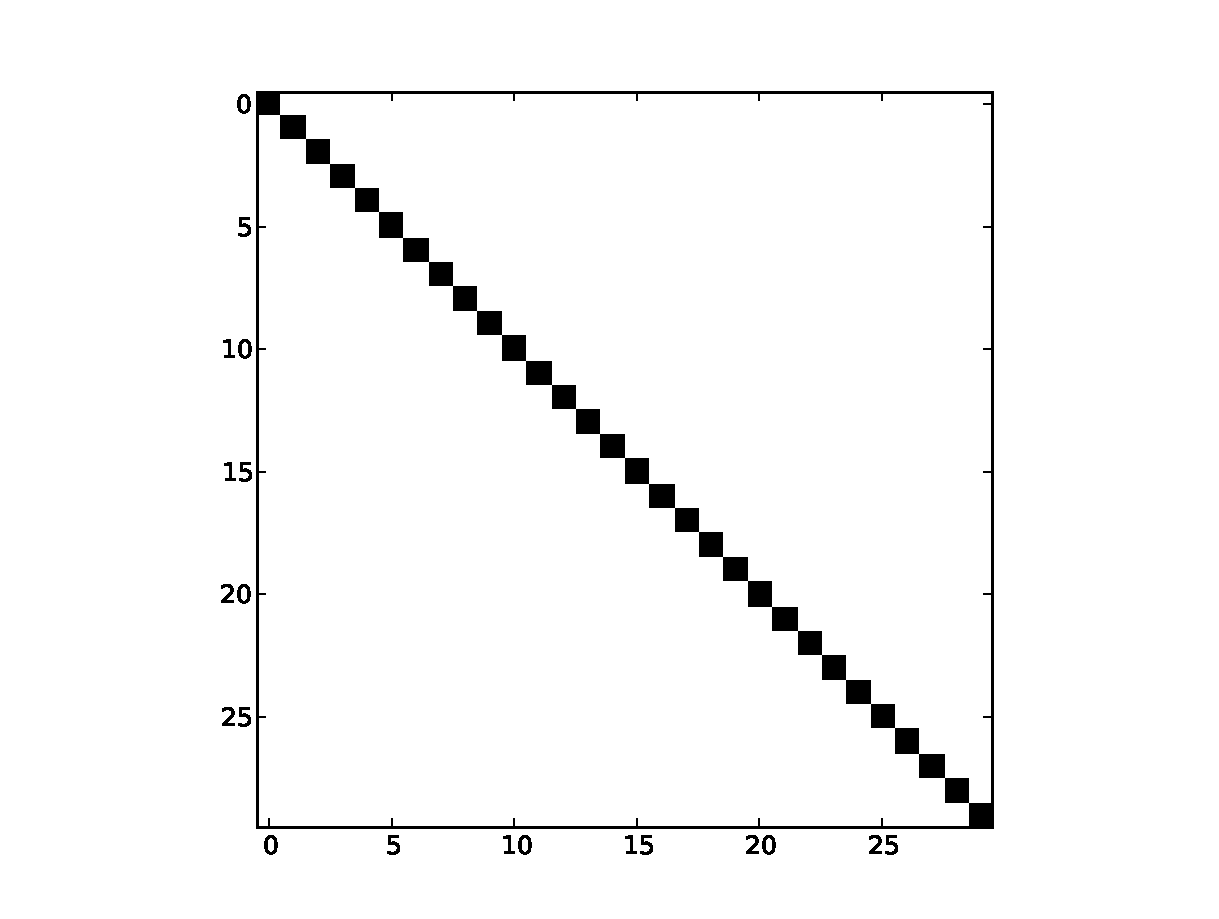
\includegraphics[width=0.5\textwidth]{figures/oneToOne}
    \caption[oneToOne mask]{\label{fig:oneToOne}
      \expr{oneToOne}
    }
  \end{center}
\end{figure}
\pagebreak
The default portion displayed by "show" is (0, 29) x (0, 29).
(0, 99) x (0, 99) can be displayed using:

\begin{code}{}
  show (oneToOne, 100, 100)
\end{code}

If source and target set is the same, oneToOne describes
self-connections.  We can use CSA to compute the set of connections
consisting of all possible connections except for self-connections
using the set difference operator "-" (Figure \ref{fig:setDifference}):

\begin{code}{}
  show (full - oneToOne)
\end{code}

\begin{figure}
  \begin{center}
    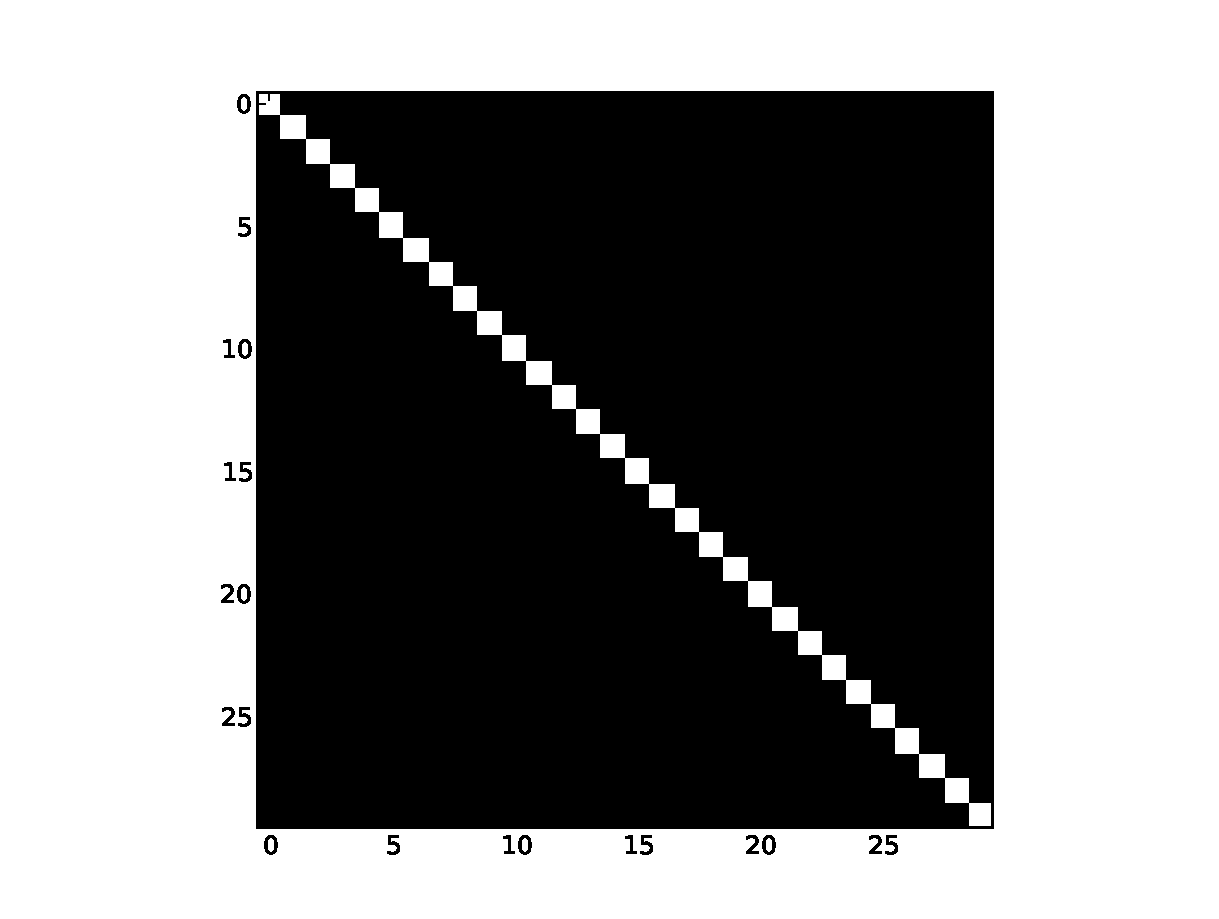
\includegraphics[width=0.5\textwidth]{figures/setDifference}
    \caption[Set difference]{\label{fig:setDifference}
      \expr{full - oneToOne}
    }
  \end{center}
\end{figure}

Finite connection sets can be represented using either lists of
connections, with connections represented as tuples (Figure
\ref{fig:twoPoints}):

\begin{code}{}
  show ([(22, 7), (8, 23)])
\end{code}

\begin{figure}
  \begin{center}
    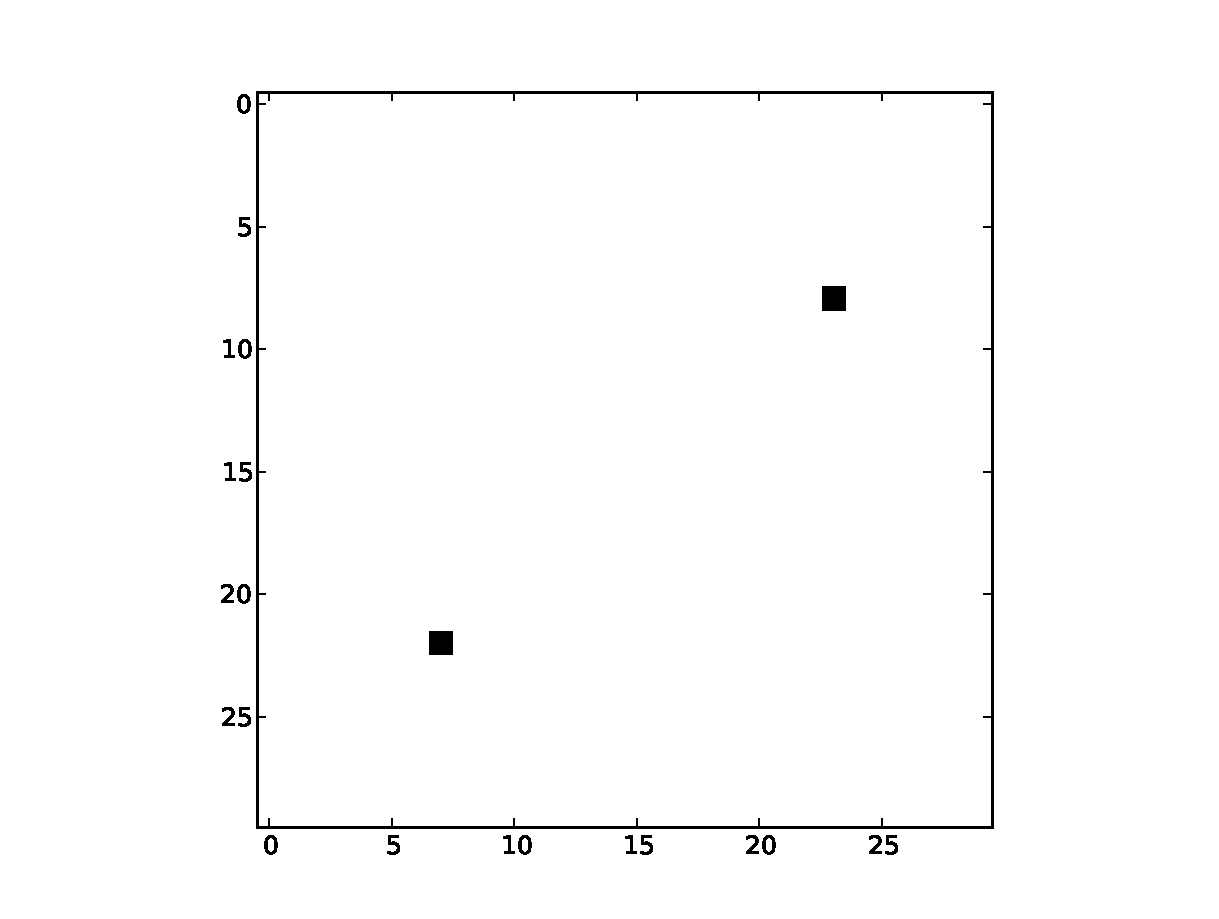
\includegraphics[width=0.5\textwidth]{figures/twoPoints}
    \caption[Mask with two connections]{\label{fig:twoPoints}
      \expr{[(22, 7), (8, 23)]}
    }
  \end{center}
\end{figure}

or using the Cartesian product of intervals (Figure \ref{fig:cartesian}):

\begin{code}{}
  show (cross (xrange (10), xrange (20)))
\end{code}

\begin{figure}
  \begin{center}
    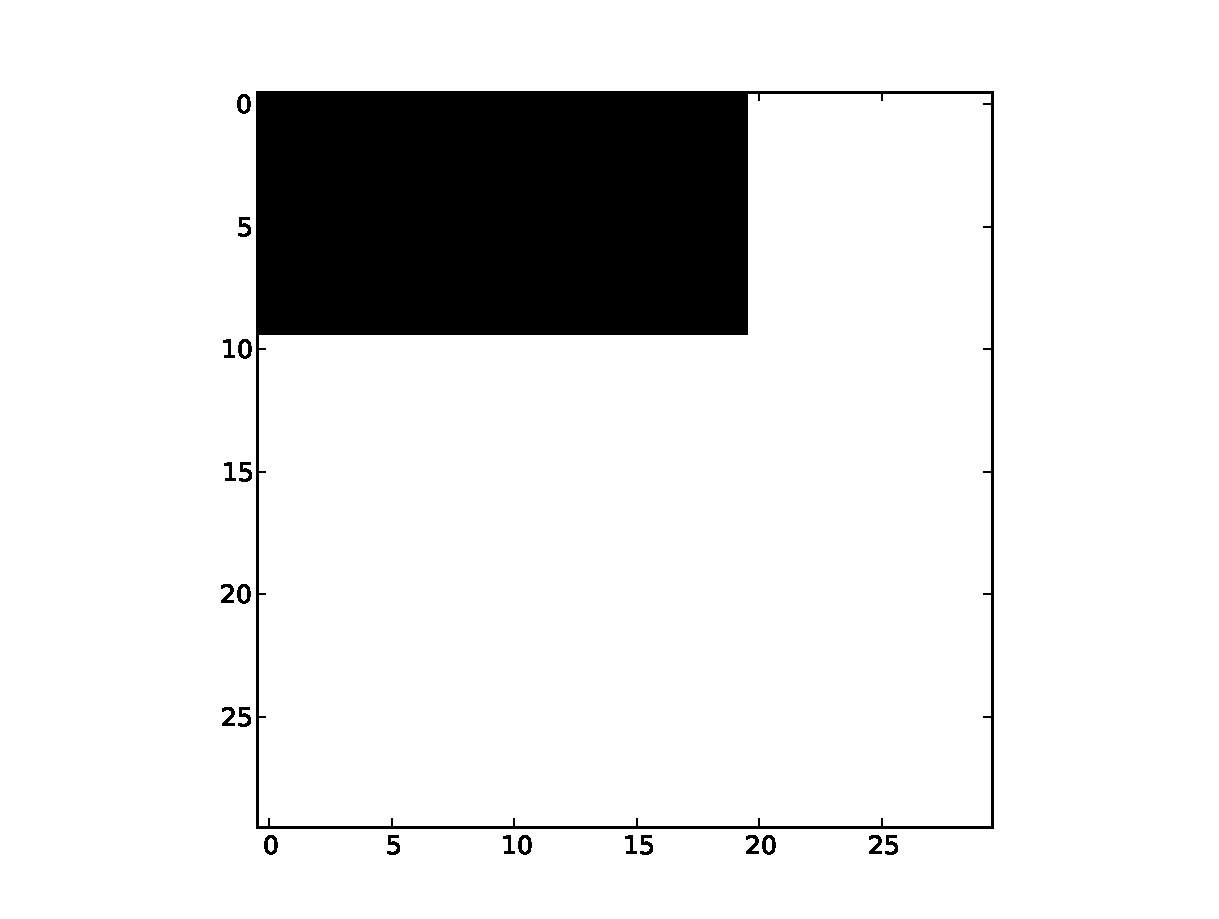
\includegraphics[width=0.5\textwidth]{figures/cartesian}
    \caption[Cartesian mask]{\label{fig:cartesian}
      \expr{xrange (10), xrange (20)}
    }
  \end{center}
\end{figure}
\pagebreak
We can form a finite version of the infinite oneToOne by taking the
intersection "*" with a finite connection set (Figure \ref{fig:intersection}):

\begin{code}{}
  c = cross (xrange (10), xrange (10)) * oneToOne
  show (c)
\end{code}

\begin{figure}
  \begin{center}
    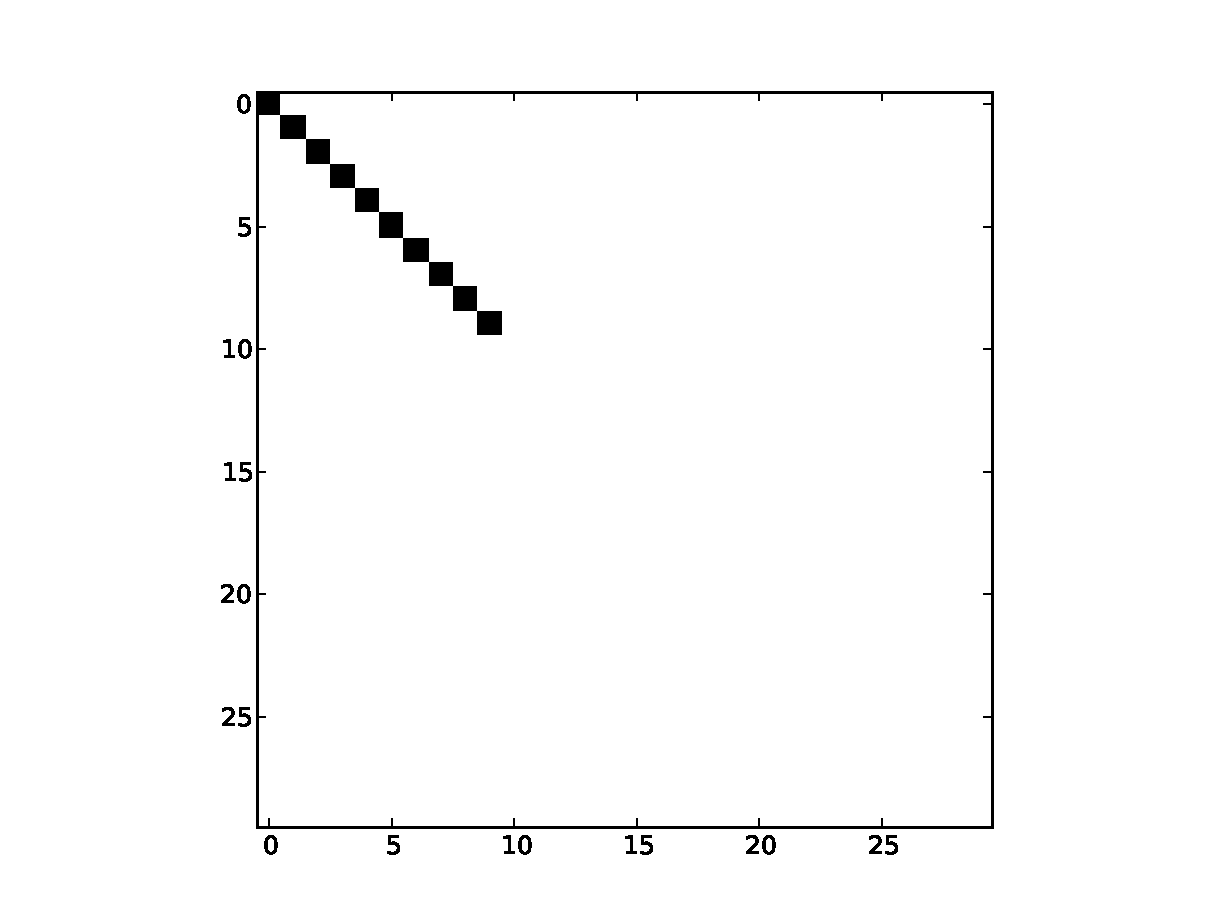
\includegraphics[width=0.5\textwidth]{figures/intersection}
    \caption[Finite part of infinite set]{\label{fig:intersection}
      \expr{cross (xrange (10), xrange (10)) * oneToOne}
    }
  \end{center}
\end{figure}

Finite connection sets can be tabulated:

\begin{code}{}
  >>> tabulate(c)
  0       0
  1       1
  2       2
  3       3
  4       4
  5       5
  6       6
  7       7
  8       8
  9       9      
\end{code}
\pagebreak
In Python, finite connection sets provide an iterator interface:

\begin{code}{}
  >>> for x in cross (xrange (4), xrange (4)) * oneToOne:
  ...   print x
  ... 
  (0, 0)
  (1, 1)
  (2, 2)
  (3, 3)
\end{code}

\section{Random connectivity}

Connectivity where the existence of each possible connection is
determined by a Bernoulli trial with probability p is expressed with
the random mask random (p), e.g. (Figure \ref{fig:random}):

\begin{code}{}
  show (random (0.5))
\end{code}

\begin{figure}
  \begin{center}
    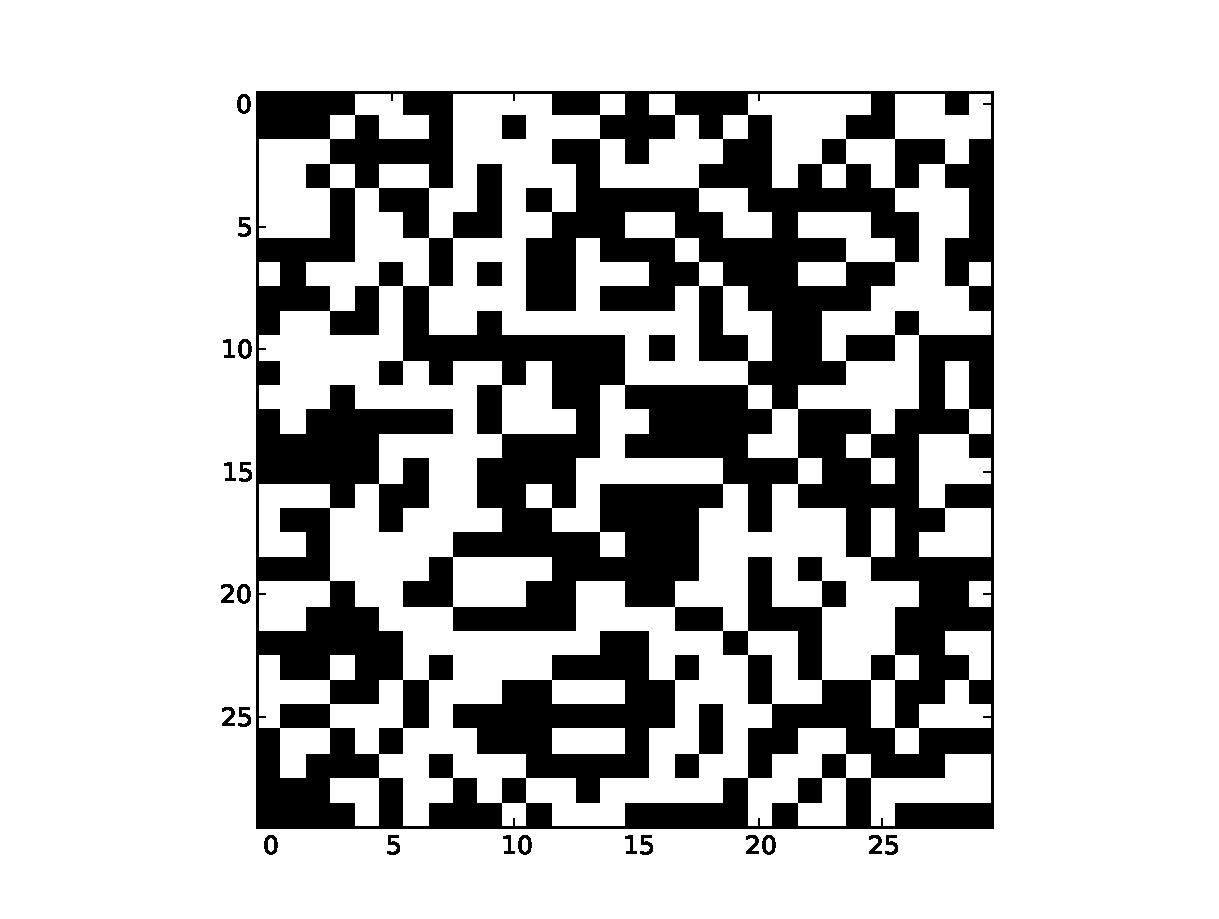
\includegraphics[width=0.5\textwidth]{figures/random}
    \caption[Random mask]{\label{fig:random}
      \expr{random (0.5)}
    }
  \end{center}
\end{figure}

\section{The block operator}
The block operator expands each connection in the operand into a
rectangular block in the resulting connection matrix, e.g. (Figure \ref{fig:blockRandom}):

\begin{code}{}
  show (block (5,3) * random (0.5))
\end{code}

\begin{figure}
  \begin{center}
    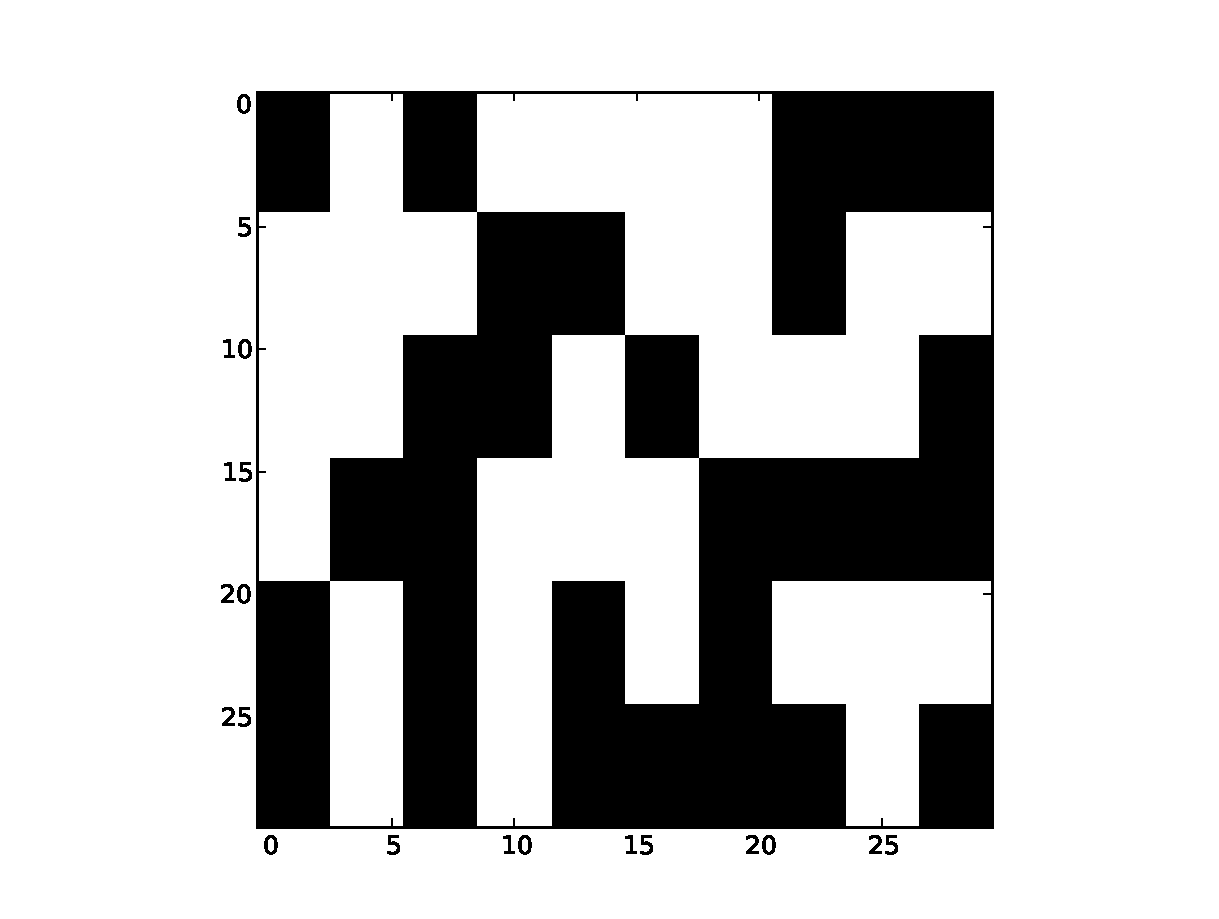
\includegraphics[width=0.5\textwidth]{figures/blockRandom}
    \caption[Block expanded random mask]{\label{fig:blockRandom}
      \expr{block (5,3) * random (0.5)}
    }
  \end{center}
\end{figure}

Note that "*" here means operator application (see section
\ref{sec:opap}).  There is also a quadratic version of the operator:

\begin{code}{}
  show (block (10) * random (0.7))
\end{code}

Using intersection and set difference, we can now formulate a more
complex mask:

\begin{code}{}
  show (block (10) * random (0.7) * random (0.5) - oneToOne)
\end{code}

\begin{figure}
  \begin{center}
    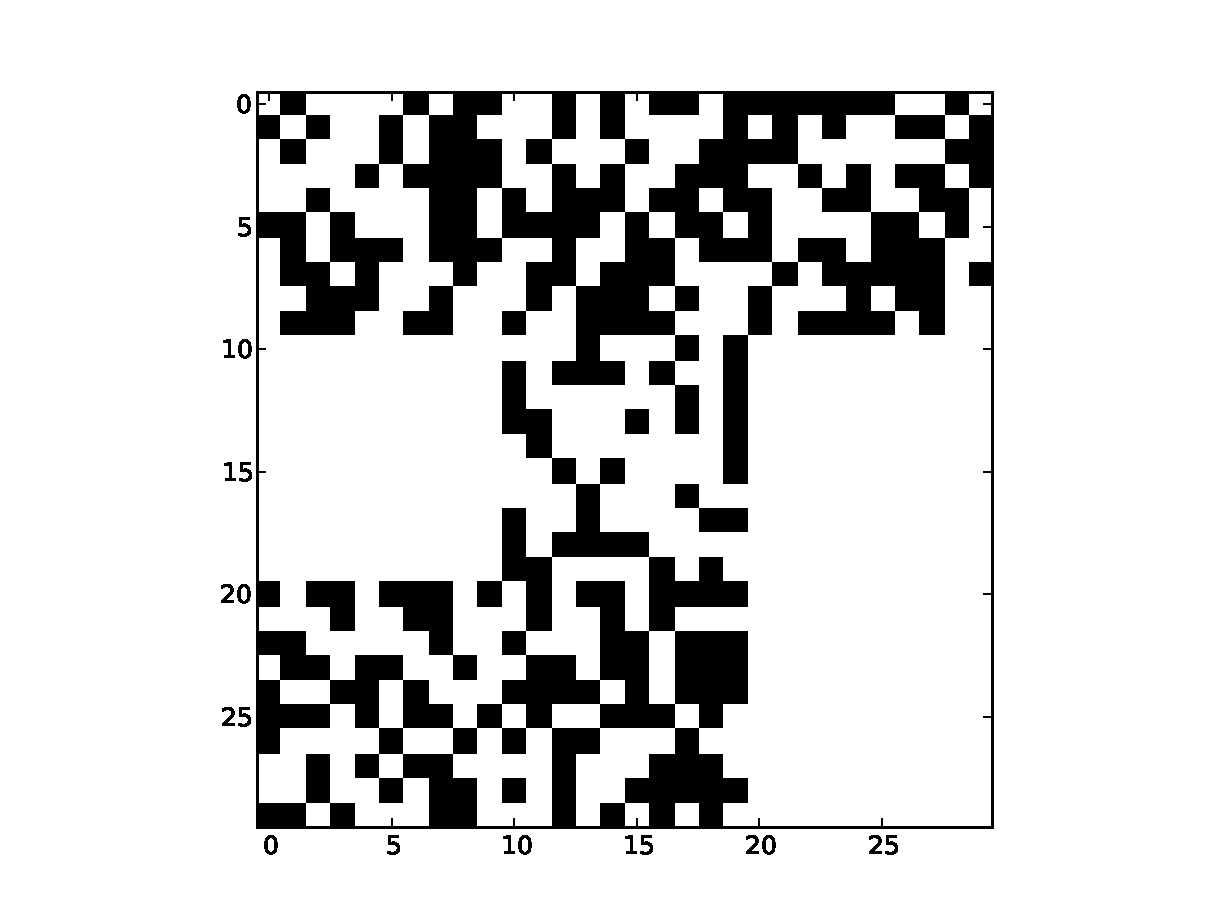
\includegraphics[width=0.5\textwidth]{figures/brro}
    \caption[Random mask]{\label{fig:brro}
      \expr{block (10) * random (0.7) * random (0.5) - oneToOne}
    }
  \end{center}
\end{figure}

The block operator is especially useful when creating connectivity
with hierarchical substructure, such as a set of cortical columns.

\section{Geometry}

In CSA, the basic tool to handle distance dependent connectivity is
metrics.  Metrics are value sets d (i, j).  Metrics can be defined
through geometry functions.  A geometry function maps an index to a
position.  We can, for example, assign a random position in the unit
square to each index:

\begin{code}{}
  g = random2d (900)
\end{code}

The positions of the grid described by g have indices from 0 to 899
and can be displayed like this:

\begin{code}{}
  gplot2d (g, 900)
\end{code}

\begin{figure}
  \begin{center}
    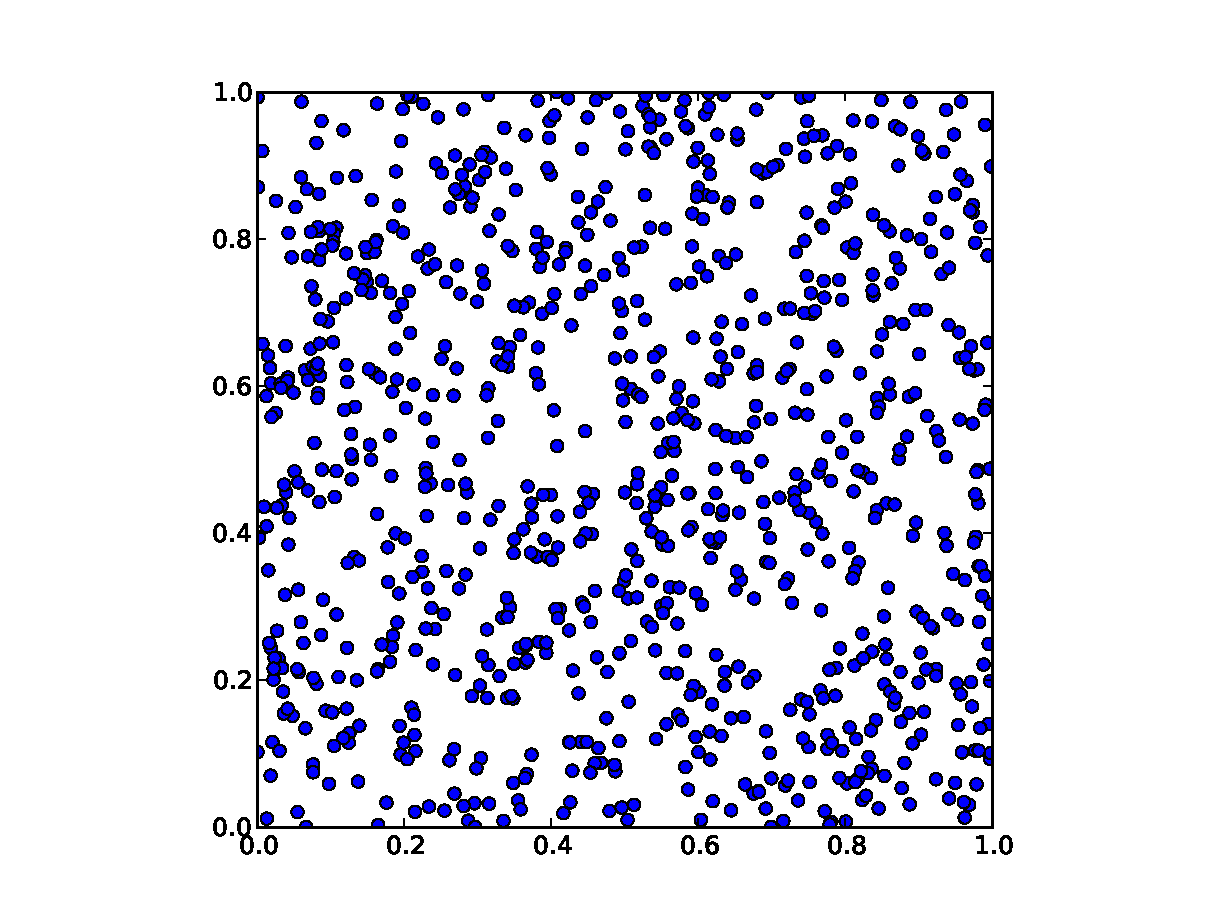
\includegraphics[width=0.5\textwidth]{figures/random2d}
    \caption[Random geometry]{\label{fig:random2d}
      \expr{gplot2d (random2d (900), 900)}
    }
  \end{center}
\end{figure}

Alternatively, we can arrange indices in a 30 x 30 grid within the
unit square:

\begin{code}{}
  g = grid2d (30)
\end{code}

\begin{figure}
  \begin{center}
    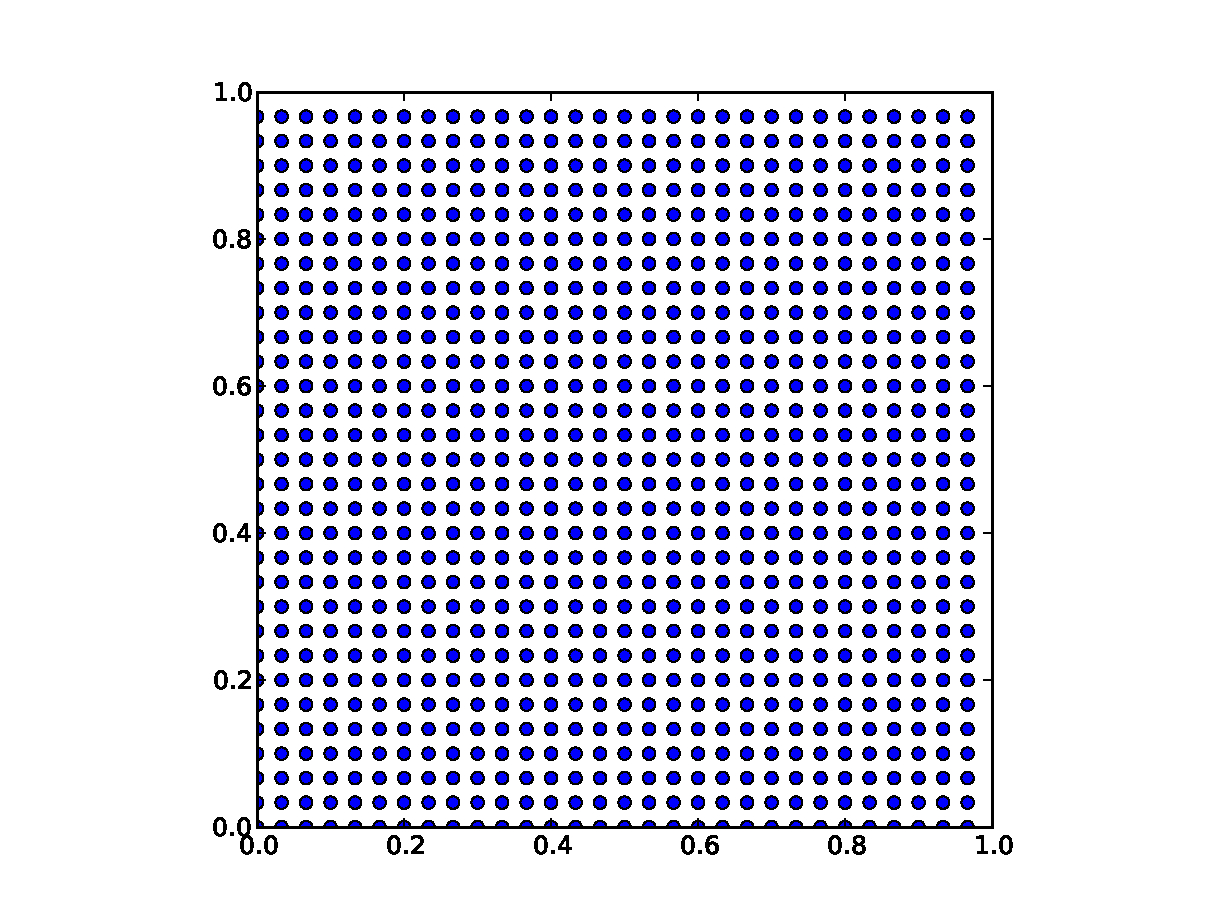
\includegraphics[width=0.5\textwidth]{figures/grid2d}
    \caption[Random geometry]{\label{fig:grid2d}
      \expr{gplot2d (grid2d (30), 900)}
    }
  \end{center}
\end{figure}

We can now define the euclidean metric on this grid:

\begin{code}{}
  d = euclidMetric2d (g)
\end{code}

An example of a distance dependent connection set is the disc mask
Disc (r) * d which connects each index i to all indices j within a
distance d (i, j) < r:

\begin{code}{}
  c = disc (r) * d
\end{code}

To examine the result we can employ the function gplotsel2d (g, c, i)
which displays the targets g (j) of i in the connection set c (Figure
\ref{fig:disc}):

\begin{code}{}
  gplotsel2d (g, c, 434)
\end{code}
\noindent [A known bug in the current implementation makes the above
  expression crash.  This only happens for infinite sets like \expr{c}
  and can be amended by intersecting it with a finite set: \expr{cross
    (xrange (900), xrange (900)) * c}.]

\begin{figure}
  \begin{center}
    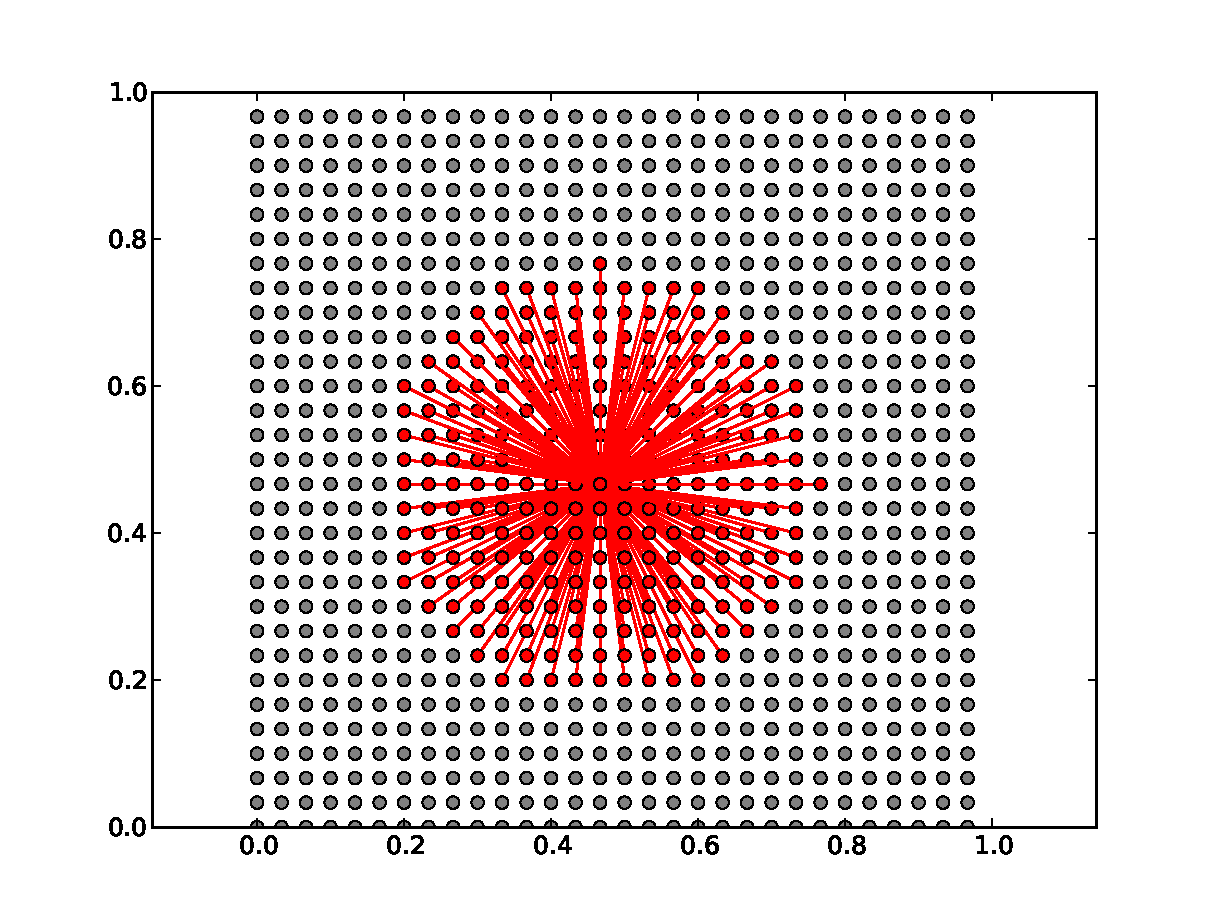
\includegraphics[width=0.5\textwidth]{figures/disc}
    \caption[Disc geometry]{\label{fig:disc}
      Projection from source neuron \#434 in \expr{disc (0.3) * d}.
    }
  \end{center}
\end{figure}

In the case where the connection set represents a projection between
two different coordinate systems, we define one geometry function for
each.  In the following example \expr{g1} is direction in visual space
in arc minutes while \expr{g2} is position in the cortical
representation of the Macaque fovea in mm:

\begin{code}{}
  g1 = grid2d (30)
  g2 = grid2d (30, x0 = -7.0, xScale = 8.0, yScale = 8.0)
\end{code}

We now define a projection operator which takes visual coordinates
into cortical (Dow et al. 1985):

\begin{code}{}
  import cmath

  @ProjectionOperator
  def GvspaceToCx (p):
      w = 7.7 * cmath.log (complex (p[0] + 0.33, p[1]))
      return (w.real, w.imag)
\end{code}

To see how the grid g1 is transformed into cortical space, we type:

\begin{code}{}
  gplot2d (GvspaceToCx * g1, 900)
\end{code}

\begin{figure}
  \begin{center}
    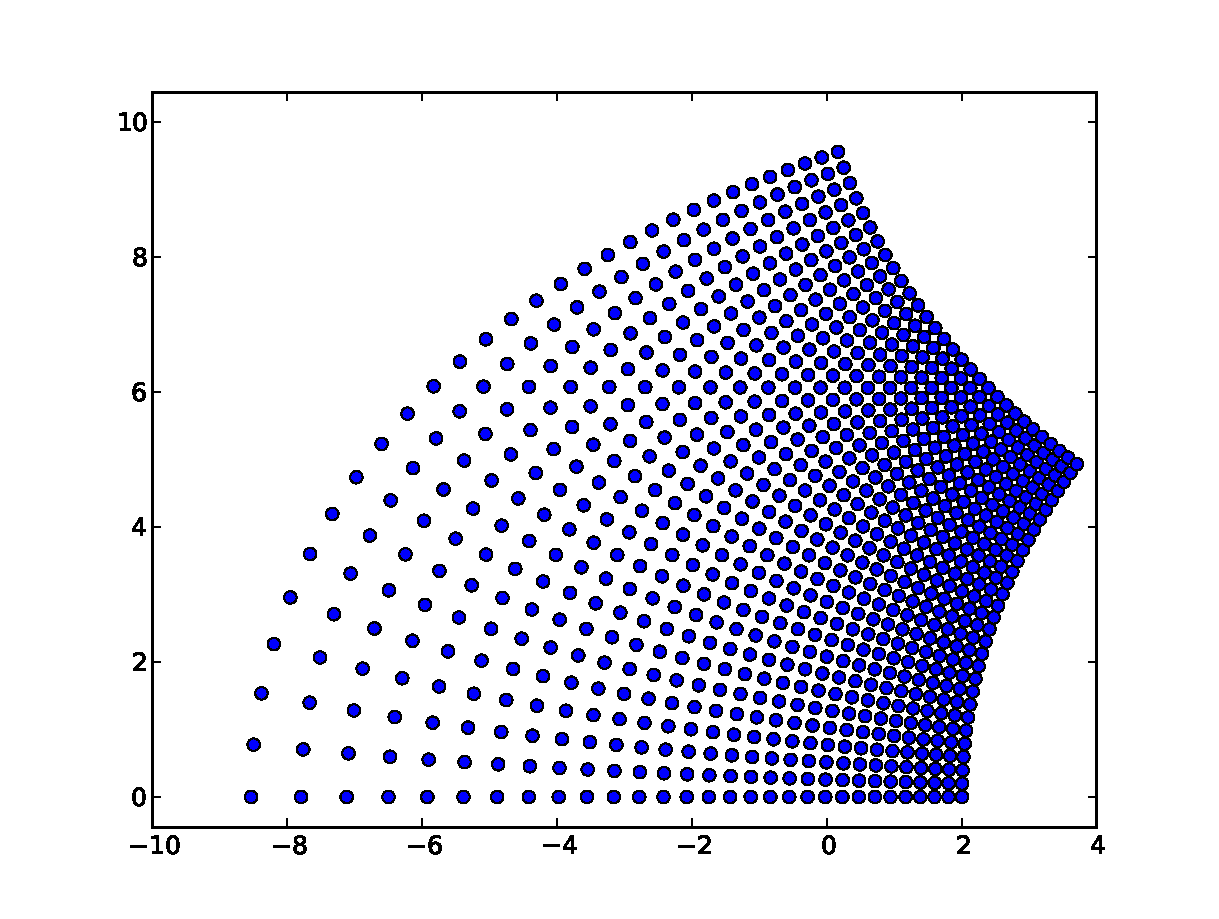
\includegraphics[width=0.5\textwidth]{figures/projection}
    \caption[Logarithmic projection]{\label{fig:projection}
      \expr{gplot2d (GvspaceToCx * g1, 900)}
    }
  \end{center}
\end{figure}

The inverse projection is defined:

\begin{code}{}
  @ProjectionOperator
  def GcxToVspace (p):
      c = cmath.exp (complex (p[0], p[1]) / 7.7) - 0.33
      return (c.real, c.imag)
\end{code}

Real receptive field sizes vary with eccentricity.  Assume, for now,
that we want to connect each target index to sources within a disc of
constant radius.  We then need to project back into visual space and
use the disc operator:

\begin{code}{}
  c = disc (0.1) * euclidMetric2d (g1, GcxToVspace * g2)
\end{code}

Again, we use gplotsel2d to check the result (Figure \ref{fig:visualDisc}):

\begin{code}{}
  gplotsel2d (g2, c, 282)
\end{code}

\begin{figure}
  \begin{center}
    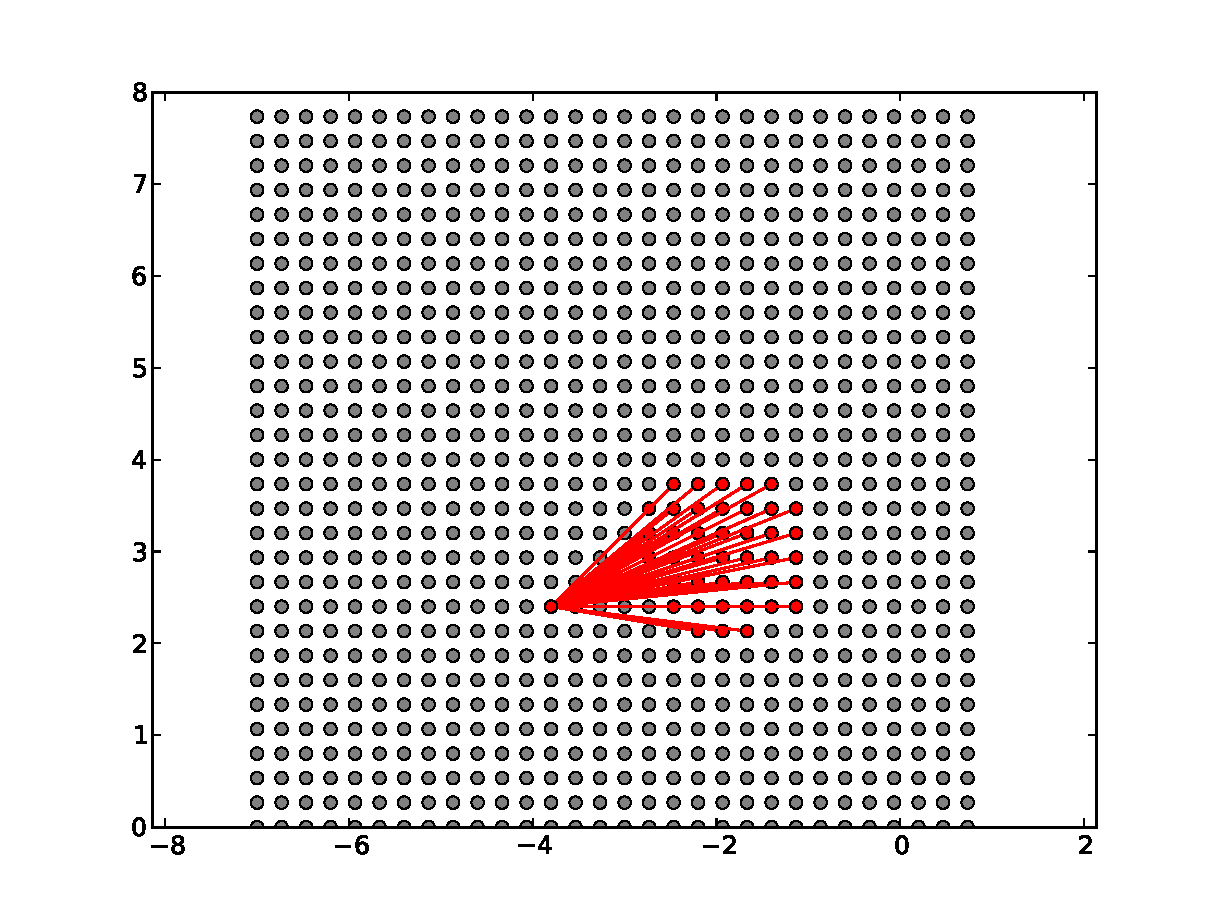
\includegraphics[width=0.5\textwidth]{figures/visualDisc}
    \caption[Random geometry]{\label{fig:visualDisc}
      \expr{disc (0.1) * euclidMetric2d (g1, GcxToVspace * g2)}
    }
  \end{center}
\end{figure}
\clearpage
\pagebreak
\section{A network with gaussian connectivity}
In the following example we represent the connectivity of a network
with excitatory and inhibitory neurons and gaussian connectivity in a
random geometry using a single connection-set (Figure \ref{fig:gaussnet}).

\begin{code}{Network with gaussian geometry-dependent connectivity}
from csa import *

# Create index intervals for excitatory, inhibitory
# and all cells
e = ival (0, 599)
i = ival (600, 899)
a = e + i

# Create geometry function g and metric d
g = random2d (900)
d = euclidMetric2d (g)

# Excitatory and inhibitory conductances, computed as
# gaussian value sets (provides the gaussian of the
# distance for every index pair)
g_e = gaussian (0.1, 0.3) * d
g_i = gaussian (0.2, 0.3) * d

# Create connection-sets with gaussian dependent random
# masks, gaussian dependent conductance and distance
# dependent delay: (mask, conductance, delay)
c_e = cset (random * g_e, g_e, d)
c_i = cset (random * g_i, -g_i, d)

# Combine excitatory and inhibitory connectivity into one
# network using intersection (*) and multiset sum (+)
# operators
c = cross (e, a) * c_e + cross (i, a) * c_i

# We may also plot the outgoing connections from one
# excitatory neuron around coordinate (0.33, 0.5) and one
# inhibitory neuron around coordinate (0.67, 0.5)
sources = [g.inverse(0.33,0.5,e), g.inverse(0.67,0.5,i)]
gplotsel2d (g, c, sources, value=0, range=[-1,1])
\end{code}

\begin{figure}
  \begin{center}
    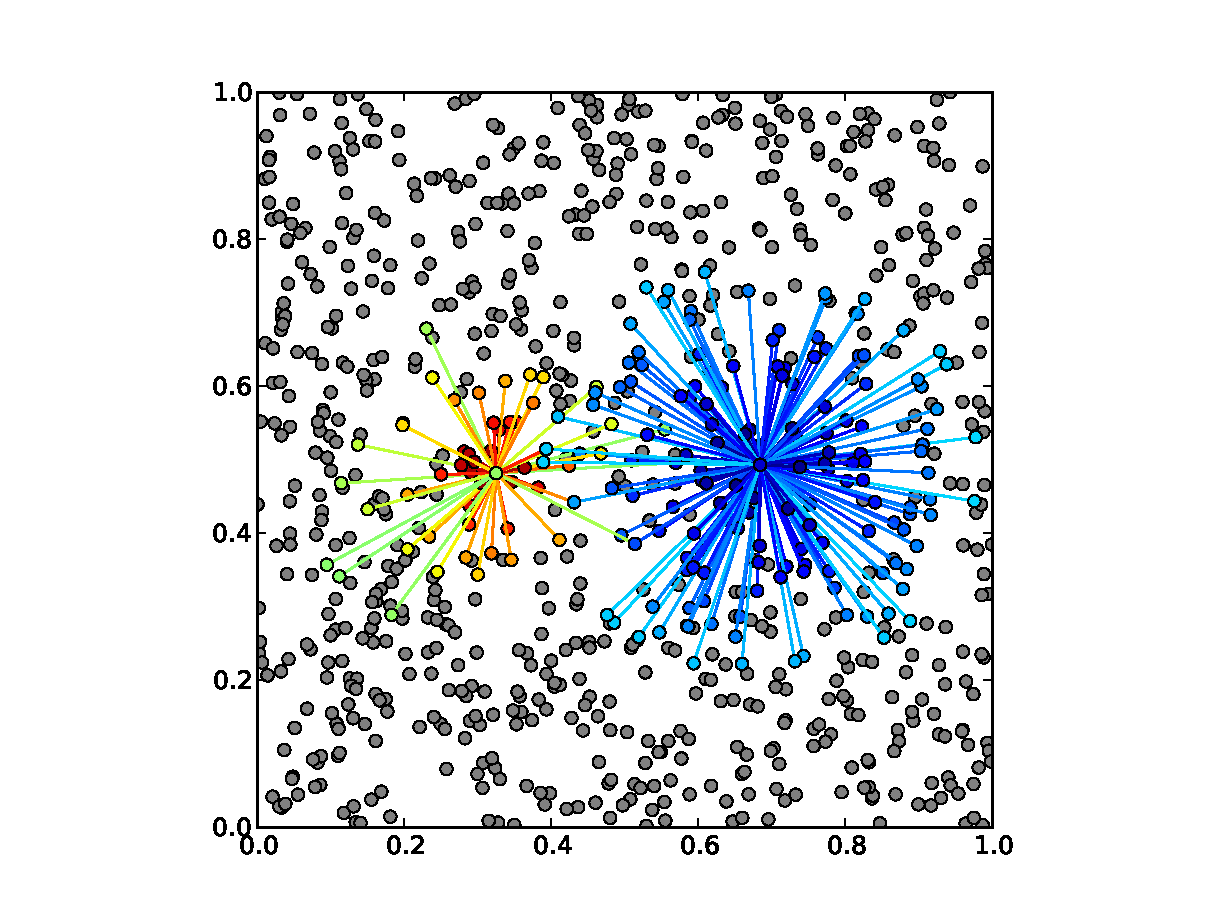
\includegraphics[width=0.9\textwidth]{figures/gaussnet}
    \caption[Projections of an excitatory and an inhibitory neuron]{\label{fig:gaussnet}
      Projections of an excitatory (warm colors) and an inhibitory
      (cold colors).
    }
  \end{center}
\end{figure}

\chapter{Reference}\label{sec:reference}

%\begin{head}{}
%\end{head}
%\begin{parameters}
%  \lstinline|| &%
%  \\
%  \lstinline|| &%
%  \\
%  \ret &%
%  \\
%\end{parameters}

This section documents how to use existing python-csa classes.

\section{Classes}
This section briefly documents some important classes in the
python-csa implementation and their public API.  The examples use many
elements which are defined in later sections.  It is suggested to use
the index on page \pageref{sec:index} to find the reference
documentation for these elements.

\subsection{ConnectionSet}\index{ConnectionSet}
A connection-set can be regarded as a set of connections, represented
by their source and target indices, with zero or more associated
values.  In the CSA, a connection-set with no associated values is a
mask.  Thus, in the python-csa implementation, in all cases where an
instance of the class \cls{ConnectionSet} is expected, it is OK to
pass an instance of \cls{Mask}.

\begin{head}{__len__}
  __len__ (self)
\end{head}
\begin{parameters}
  \ret &%
  the number of connections in this connection-set\\
\end{parameters}
This method returns the number of connections in this connection-set.
An error is reported if this connection-set isn't finite.
\begin{code}{Obtaining the number of connections in a connection-set}
>>> len (cross ((0, 1), (0, 1)))
4
\end{code}

\begin{head}{__iter__}
  __iter__ (self)
\end{head}
\begin{parameters}
  \ret &%
  iterator over the connections represented by this instance\\
\end{parameters}
This method returns an iterator over the connections represented by
this instance.  Each item generated by the iterator is a tuple
\[ (i, j, v_0, ..., v_{n-1}) \]
\begin{code}{Iterating over a connection-set}
>>> m = cross ((0, 1), (2, 3))
>>> v = vset (lambda i, j: i + j)
>>> c = cset (m, v, v * v)
>>> for x in c:
...   print x
... 
(0, 2, 2, 4)
(1, 2, 3, 9)
(0, 3, 3, 9)
(1, 3, 4, 16)
\end{code}

\subsection{Mask}\index{Mask}
A mask gives information about which connections exist.  It can be
regarded as a set of connections, represented by their source and
target indices.  In the CSA, a connection-set with no associated
values is a mask.  In the python-csa implementation, an attempt to
construct a connection-set with zero associated values, yields an
instance of the class \cls{Mask}.  In cases where a mask is expected,
a python list of (source, target) tuples can also be passed.

The class \cls{Mask} has the same public methods (\expr{__len__},
\expr{__iter__}) as the class \cls{ConnectionSet}.

\subsection{ValueSet}\index{ValueSet}
To be documented.

\subsection{IntervalSet}\index{IntervalSet}\label{sec:intervalset}
To be documented.

\section{Constructor and selectors}

\subsection{cset}\index{cset}

\begin{head}{cset}
  cset (mask, valueSet, ...)
\end{head}
\begin{parameters}
  \lstinline|mask| &%
  a \lstinline|Mask| \\
  \lstinline|valueSet| &%
  zero or more \lstinline|ValueSet|:s \\
\end{parameters}
This function constructs and returns a connection-set from a
\lstinline|Mask| and zero or more \lstinline|ValueSet|:s.  [Note: In
  the current implementation, \lstinline|mask| is returned if no
  value-sets are given.  This should probably change so that a new
  object is returned.]

\subsection{mask}\index{mask}

\begin{head}{mask}
  mask (cset)
\end{head}
\begin{parameters}
  \lstinline|cset| &%
  a \lstinline|ConnectionSet|\\
  \emph{return value} &%
  the \lstinline|Mask| of \lstinline|cset|\\
\end{parameters}
This function returns the \lstinline|Mask| of the
\lstinline|ConnectionSet| \lstinline|cset|.

\subsection{value}\index{value}

\begin{head}{value}
  value (cset, k)
\end{head}
\begin{parameters}
  \lstinline|cset| &%
  a \lstinline|ConnectionSet|\\
  \lstinline|k| &%
  index of the value-set to return\\
  \emph{return value} &%
  the \lstinline|k|:th \lstinline|ValueSet| of \lstinline|cset|\\
\end{parameters}
This function returns the \lstinline|k|:th \lstinline|ValueSet| of the
\lstinline|ConnectionSet| \lstinline|cset|.

\subsection{arity}\index{arity}

\begin{head}{arity}
  arity (cset)
\end{head}
\begin{parameters}
  \lstinline|cset| &%
  a \lstinline|ConnectionSet|\\
  \emph{return value} &%
  the \emph{arity} of \lstinline|cset|\\
\end{parameters}
This function returns the \emph{arity} of the
\lstinline|ConnectionSet| \lstinline|cset|.  The arity of a
connection-set is the number of value-sets of the connection-set.

\subsection{vset}\index{vset}

\begin{head}{vset}
  vset (x)
  vset (callable)
\end{head}
\begin{parameters}
  \lstinline|x| &%
  a value\\
  \lstinline|callable| &%
  a callable taking two arguments\\
\end{parameters}
This function constructs and returns a value-set.  In the first form,
the number \fa{x} is taken as the value of each of all existing
connections.  In the second form, the value of each existing
connection is the one returned by applying \fa{callable} to the source
and target indices of the connection.

\section{Integer sets}
In the current python-csa implementation, integer sets are usually
represented using the class \cls{IntervalSet} (see section
\ref{sec:intervalset}).  Functions that take integer sets as arguments
generally coerce \cls{tuple}:s of two non-negative integers into
\cls{IntervalSet}:s:
\begin{code}{}
  (1, 2) --> IntervalSet ([(1,2)])
\end{code}

\subsection{ival}\index{ival}

\begin{head}{ival}
  ival (beginning, end)
\end{head}
\begin{parameters}
  \lstinline|beginning| &%
  start of interval\\
  \lstinline|end| &%
  end of interval (inclusive)\\
  \emph{return value} &%
  the interval \lstinline|(beginning, end)|\\
\end{parameters}
This function returns the interval \lstinline|(beginning, end)|
represented as a set of non-negative integers.  The underlying
representation is space-efficient.

\subsection{N}\index{N}

\begin{head}{N}
  N
\end{head}
\begin{parameters}
\end{parameters}
This constant represents the set of all non-negative integers.

\subsection{cross}\index{cross}

\begin{head}{cross}
  cross (set0, set1)
\end{head}
\begin{parameters}
  \lstinline|set0| &%
  a set of non-negative integers\\
  \lstinline|set1| &%
  a set of non-negative integers\\
  \emph{return value} &%
  the Cartesian cross product of \fa{set0} and \fa{set1}\\
\end{parameters}
This function returns the Cartesian cross product of \fa{set0} and
\fa{set1} represented as a \cls{Mask}.

\begin{code}{The Cartesian product of (1,2) and (3,4)}
>>> tabulate (cross ((1,2), (3,4)))
1 	3
2 	3
1 	4
2 	4
\end{code}

\section{Utilities}

\begin{head}{tabulate}
  tabulate (cset)
\end{head}
\begin{parameters}
  \lstinline|cset| &%
  a \cls{ConnectionSet}\\
\end{parameters}
This procedure tabulates the connection-set \fa{cset}.  An iteration
over the connections in \fa{cset} is performed.  The source and target
indices are tabulated in the first and second columns with value-sets
tabulated in columns three and upwards.

Tabulate can be used to print connection-sets during development.

\section{Elementary masks}

\subsection{empty}\index{empty}

\begin{head}{empty}
  empty
\end{head}
\begin{parameters}
\end{parameters}
This constant \cls{Mask} represents the set of no connection.
Iterating results in nothing, no matter how hard you try.

\subsection{full}\index{full}

\begin{head}{full}
  full
\end{head}
\begin{parameters}
\end{parameters}
This constant \cls{Mask} represents the (infinite) set of all
connections.

\begin{code}{Finite portion of the \expr{full} mask}
>>> tabulate (cross ((0, 1), (0, 1)) * full)
0 	0
1 	0
0 	1
1 	1
\end{code}

\subsection{oneToOne}\index{oneToOne}
\begin{head}{oneToOne}
  oneToOne
\end{head}
\begin{parameters}
\end{parameters}
This constant \cls{Mask} represents the (infinite) set of one-to-one
connections.  It resembles Kronecker's delta or an infinite identity
matrix.

\begin{code}{Finite portion of the \expr{oneToOne} mask}
>>> tabulate (cross ((0, 3), (0, 3)) * oneToOne)
0 	0
1 	1
2 	2
3 	3
\end{code}

\subsection{random}\index{random}
\begin{head}{random}
  random (p)
\end{head}
\begin{parameters}
  \lstinline|p| &%
  the probability for a potential connection to exist\\
  \ret &%
  an infinite \cls{Mask} where the existence of each connection is
  determined by a Bernoulli trial with probability \fa{p}.\\
\end{parameters}
This function returns a random mask where a connection between given
source and target indices exists with probability \fa{p}.

See also section \ref{sec:randomop} for the set of functions returning
random \emph{operators}.  These support sampling a given number of
connections from a finite mask or random sampling with constraints on
\fa{fanIn} or \fa{fanOut}.

\section{Set operators}
The following binary operators can be applied to integer sets,
masks and connection-sets:
\par\vspace{4mm}\hrule\par\vspace{1mm}
\begin{tabular}{@{\hspace{2em}}lp{0.6\textwidth}}
  \expr{A + B} & the \emph{multiset sum} of A and B\\
  \expr{A - B} & the \emph{set difference} between A and B\\
  \expr{A * B} & the \emph{intersection} of A and B\\
\end{tabular}\par\vspace{1mm}\par\hrule\par\vspace{5mm}

In addition, the following unary operator applies to integer sets and masks:
\par\vspace{4mm}\hrule\par\vspace{1mm}
\begin{tabular}{@{\hspace{2em}}lp{0.6\textwidth}}
  \expr{\~A} & the \emph{complement} of A\\
\end{tabular}\par\vspace{1mm}\par\hrule\par\vspace{5mm}

\section{Arithmetic operators}
The arithmetic operators on connection-sets which are defined in the
connection-set algebra are not yet implemented in the python-csa demo
implementation.

\section{Operator application}\label{sec:opap}
The operator application operator is used to apply unary
connection-set algebra operators to their operand:
\par\vspace{4mm}\hrule\par\vspace{1mm}
\begin{tabular}{@{\hspace{2em}}lp{0.6\textwidth}}
  \expr{operator * operand} & apply \fa{operator} to \fa{operand}\\
\end{tabular}\par\vspace{1mm}\par\hrule\par\vspace{5mm}
The operator application operator is overloaded with the arithmetic
multiplication and set intersection operators.

\section{Miscellaneous connection-set operators}\label{sec:miscop}

\subsection{random}\index{random}\label{sec:randomop}
\begin{head}{random}
  random (N = n) * cset
\end{head}
\begin{parameters}
  \lstinline|n| &%
  the number of connections to sample (keyword arg named \fa{N})\\
  \fa{cset} &%
  any \emph{finite} connection-set\\
  \ret &%
  a connection-set containing \fa{n} randomly sampled connections from
  \fa{cset}\\
\end{parameters}

\begin{head}{random}
  random (fanIn = n) * cset
\end{head}
\begin{parameters}
  \lstinline|n| &%
  the number of sources sampled for each target (keyword arg named \fa{fanIn})\\
  \fa{cset} &%
  any \emph{finite} connection-set\\
  \ret &%
  a connection-set randomly sampled from \fa{cset} with fanIn \fa{n}\\
\end{parameters}

\begin{head}{random}
  random (fanOut = n) * cset
\end{head}
\begin{parameters}
  \lstinline|n| &%
  the number of targets sampled for each source (keyword arg named \fa{fanOut})\\
  \fa{cset} &%
  any \emph{finite} connection-set\\
  \ret &%
  a connection-set randomly sampled from \fa{cset} with fanOut \fa{n}\\
\end{parameters}

\subsection{disc}\index{disc}

\begin{head}{disc}
  disc (r) * metric
\end{head}
\begin{parameters}
  \fa{r} & radius \\
  \ret & a mask of all connections for which
  \expr{metric (source, target) < r} \\
\end{parameters}

\subsection{gaussian}\index{gaussian}

\begin{head}{gaussian}
  gaussian (sigma, cutoff) * metric
\end{head}
\begin{parameters}
  \lstinline|sigma| &%
  \\
  \lstinline|cutoff| &%
  \\
  \ret & a value set associating the result of applying the normalized
  gaussian function with standard deviation \fa{sigma} and cutoff
  \fa{cutoff} to \expr{metric (source, target)} to each connection\\
\end{parameters}

\subsection{block}\index{block}

\begin{head}{block}
  block (M, N)
  block (M)
\end{head}
\begin{parameters}
  \fa{M} & \\
  \fa{N} & \\
\end{parameters}

\subsection{block1}\index{block1}

\begin{head}{block1}
  block1 (N)
\end{head}
\begin{parameters}
\end{parameters}

\subsection{transpose}\index{transpose}

\begin{head}{}
  transpose
\end{head}
\begin{parameters}
\end{parameters}

\subsection{shift}\index{shift}

\begin{head}{shift}
  shift (M, N)
\end{head}
\begin{parameters}
  \lstinline|M| &%
  \\
  \lstinline|N| &%
  \\
\end{parameters}

\subsection{fix}\index{fix}

\begin{head}{fix}
  fix
\end{head}
\begin{parameters}
\end{parameters}

\section{Geometry}

\subsection{grid2d}\index{grid2d}

\begin{head}{grid2d}
  grid2d (width, xScale = 1.0, yScale = 1.0, x0 = 0.0, y0 = 0.0)
\end{head}
\begin{parameters}
  \lstinline|width| &%
  \\
  \lstinline|xScale| &%
  \\
  \emph{return value} &%
  \\
\end{parameters}

\subsection{random2d}\index{random2d}

\begin{head}{random2d}
  random2d (N, xScale = 1.0, yScale = 1.0)
\end{head}
\begin{parameters}
  \lstinline|| &%
  \\
  \lstinline|| &%
  \\
  \emph{return value} &%
  \\
\end{parameters}

\subsection{euclidMetric2d}\index{euclidMetric2d}

\begin{head}{}
  euclidMetric2d (g1, [g2])
\end{head}
\begin{parameters}
  \lstinline|g1| &%
  \\
  \lstinline|g2| optional &%
  \\
  \emph{return value} &%
  \\
\end{parameters}

\subsection{ProjectionOperator}\index{ProjectionOperator}

\begin{head}{ProjectionOperator}
  @ProjectionOperator
  def fname (p):
    ...
    return q
\end{head}
\begin{parameters}
  \lstinline|fname| &%
  \\
  \lstinline|p| &%
  \\
\end{parameters}

\section{Plotting}

\subsection{show}\index{show}

\begin{head}{show}
  show (cset, N0 = 30, [N1])
\end{head}
\begin{parameters}
  \lstinline|cset| &%
  \\
  \lstinline|N0| &%
  \\
\end{parameters}

\subsection{gplotsel2d}\index{gplotsel2d}

\begin{head}{gplotsel2d}
  gplotsel2d (g, cset, source = N, target = N,
              N0 = 900, [N1], [value], range=[], lines = True)
\end{head}
\begin{parameters}
  \lstinline|| &%
  \\
  \lstinline|| &%
  \\
\end{parameters}

\begin{head}{gplot2d}
  gplot2d (g, N, [color], show = True)
\end{head}
\begin{parameters}
  \lstinline|| &%
  \\
  \lstinline|| &%
  \\
\end{parameters}

\label{sec:index}
\printindex

\end{document}


%%% Local Variables: 
%%% mode: latex
%%% TeX-master: t
%%% eval: (flyspell-mode 1)
%%% eval: (ispell-change-dictionary "american")
%%% eval: (flyspell-buffer)
%%% End: 
